\documentclass[12pt]{ctexart}
\usepackage[utf8]{inputenc}
\usepackage[T1]{fontenc}
\usepackage{graphicx}
\usepackage{xcolor}
\usepackage{minted}
\usepackage[colorlinks,linkcolor=black]{hyperref}

\usepackage{enumerate}
\usepackage{enumitem}
\setlist[enumerate,1]{label=(\arabic*).,font=\textup,
leftmargin=7mm,labelsep=1.5mm,topsep=0mm,itemsep=-0.8mm}
\setlist[enumerate,2]{label=(\alph*).,font=\textup, 
leftmargin=7mm,labelsep=1.5mm,topsep=-0.8mm,itemsep=-0.8mm}

\usepackage{colortbl}
\definecolor{tabcolor}{HTML}{7E0C6E} %三线表改成南开紫


%%novalidate

\usepackage{tikz}
\usepackage{calc}
\usepackage{booktabs}


% colors
\definecolor{color1}{HTML}{7E0C6E} % 19% Dark Blue
% \definecolor{color1}{HTML}{8C260F} % Dark red
\definecolor{color2}{HTML}{333333} % 20% gray
% \definecolor{color2}{HTML}{000060} % 19% Dark Blue
\definecolor{colorcover}{HTML}{7E0C6E} % 20% gray

% fonts
\usepackage{fontspec}
\defaultfontfeatures{Mapping=tex-text}
\setmainfont
[BoldFont=Lato-Bold.ttf,
ItalicFont=Lato-Italic.ttf,
BoldItalicFont=Lato-BoldItalic.ttf]
{Lato-Regular.ttf}
\newfontfamily\headingfont[ItalicFont=Lato-BlackItalic.ttf]{Lato-Black.ttf}
%%%

\usepackage{geometry}
\geometry{a4paper,
hmargin=20mm,vmargin=20mm,
head=0ex,foot=3ex}

\linespread{1.3}

\usepackage[hang]{caption}
\DeclareCaptionFormat{upper}{#1#2\uppercase{#3}\par}
\captionsetup{labelfont={bf,color=color2},textfont={normalsize,color=color2},format = upper,figurename=FIGURE,tablename=TABLE}

%%% fancy sections
\usepackage{titlesec}
%\titleformat{\chapter}{\headingfont\LARGE\bfseries\scshape\color{color1}}{\thechapter}{1em}{}[\titlerule]
\titleformat{\section}{\color{color1}\headingfont\Large\bfseries\uppercase}{\thesection}{1em}{}[\titlerule]
\titleformat{\subsection}{\color{color1}\headingfont\large\bfseries\uppercase}{\thesubsection}{1em}{}
\titleformat{\subsubsection}{\color{color1}\headingfont\bfseries\uppercase}{\thesubsubsection}{1em}{}
%%%

% head and foot
\usepackage{fancyhdr}
\pagestyle{fancy}
\lhead{}
\chead{}
\makeatletter
\rhead{\color{color2}\@date}
\makeatother
\newlength{\myheight}
\lfoot{
\settoheight{\myheight}{\thepage}
\raisebox{3ex-5\myheight}{
\includegraphics[height=10ex]{logo}}
}

\renewcommand\headrulewidth{0pt}
\renewcommand\footrulewidth{0pt}

%%% picture on cover page
\usepackage{eso-pic}
\newcommand\BackgroundPic{%
\put(0,0){%
\parbox[b][\paperheight]{\paperwidth}{%
\vfill
\centering
\includegraphics[width=\paperwidth,height=\paperheight,%
keepaspectratio]{cover}%
\vfill
}}
\put(0,0){%
\parbox[b][\paperheight]{\paperwidth}{%
\vfill
\centering

\includegraphics[width=0.5\paperwidth]{logo.png}%
\vfill
}}}
%%%
% custom titlepage
\makeatletter
\renewcommand{\maketitle}{
\thispagestyle{empty}
\AddToShipoutPicture*{\BackgroundPic}
\ClearShipoutPicture
%
\phantom{a}
\vfill
\phantom{a}\hfill
\begin{tabular}[c]{@{}p{0.7\textwidth}@{}}
      \color{colorcover}\headingfont\LARGE\@title\\[1em]
      \color{colorcover}\headingfont\Large\@author\\[2em]
\end{tabular}
%
\clearpage
}
\makeatother
%%%


%%% fancy boxes
\usepackage{tcolorbox}
\usepackage{wrapfig}
\def\fullboxbegin{
\bigskip
\begin{tcolorbox}[colback=color1,colframe=color1,coltext=white,arc=0mm,boxrule=0pt]
}
\def\fullboxend{\end{tcolorbox}\medskip}
%
\def\leftboxbegin{
\begin{wrapfigure}{l}{0.5\textwidth}
\begin{tcolorbox}[colback=color1,colframe=color1,coltext=white,arc=0mm,boxrule=0pt]
}
\def\leftboxend{
\end{tcolorbox}
\end{wrapfigure}
}
%
\def\rightboxbegin{
\begin{wrapfigure}{r}{0.5\textwidth}
\begin{tcolorbox}[colback=color1,colframe=color1,coltext=white,arc=0mm,boxrule=0pt]
}
\def\rightboxend{
\end{tcolorbox}
\end{wrapfigure}
}
%
\newcounter{frames}
\def\frameboxbegin#1{
\bigskip
\refstepcounter{frames}
\begin{tcolorbox}[colback=white,colframe=color1,arc=0mm,title={\MakeUppercase{\textbf{Frame \arabic{frames}}: #1}}]
}
\def\frameboxend{
\end{tcolorbox}
}
%%%


% No Hyphenation
\tolerance=1
\emergencystretch=\maxdimen
\hyphenpenalty=10000
\hbadness=10000

\usepackage{lipsum}
\usepackage{pifont}

\date{}


\begin{document}


\tableofcontents
\clearpage

\section{课程收获}

\subsection{课程知识收获}

\subsubsection{工业自动化系统及控制流程}


\rightboxbegin
sadsgfdhfdgnfdrghnhfgrzsdfvbfndhergsfdbfngdgvc bnhdfbfdb
\rightboxend

\lipsum[1]

\lipsum[1]

\begin{enumerate}
  \item \textbf{AWFS}
 
  \item \textbf{asf}
 
  \item \textbf{adfgds}
\end{enumerate}

\begin{figure}[H]
\centering
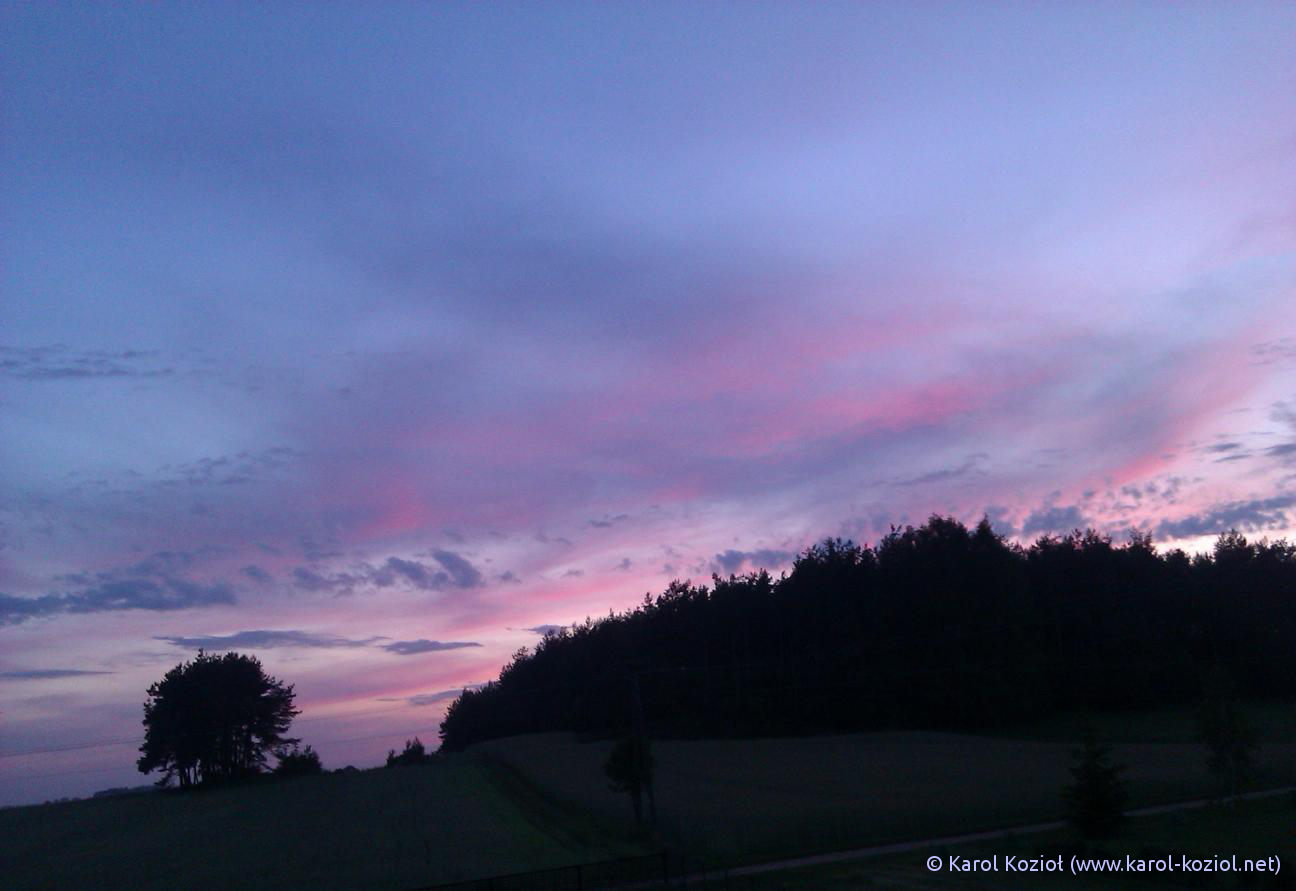
\includegraphics[width=0.45\textwidth]{sky.jpg}
\caption{sky}
\end{figure}


\lipsum[1]

\begin{table}[h]
\centering
\begin{tabular}{ccc}
\arrayrulecolor{tabcolor} \toprule[1.4pt] 
&adsgsadga & asgsdgsaag \\
\hline
sf & sd & sgsgf \\
sf & sdg & sdg \\
sdf & sdg & gfdg \\
sdf & sdg & dfg \\
sdg & dgdsf & asdgf \\

\bottomrule[1.4pt]
\end{tabular}
\caption {sdgdhghdmtjmfhgn}
\label{tab:number}
\end{table}


\subsubsection{各类被控对象的运动控制}



\subsubsection{工业PLC控制系统}


\lipsum[1]

\leftboxbegin
\begin{enumerate}
  \item fdsdxc
  \item szdndgfgbd
  \item dfxnghmukj
  \item fdbgnfhmj,k
  \item szdfbghnfmj
\end{enumerate}
\leftboxend

\lipsum[1]
\lipsum[1]
\lipsum[1]




\frameboxbegin{ex}

\textbf{[1]asfgfhrydtuj}

\qquad fdhgdasdfghjj;o



\textbf{[2]asfdgfhgj}

\qquad ghgtdjyhkfutl,mcgfngdg。

\textbf{[3]dscghfjgkhuli;}

\qquad sdfhdgjhmfkgj,lhk.u


\frameboxend

\lipsum[1]
\lipsum[1]

\begin{description}
  \item[\ding{52}] afegdsrhtjy
  \item[\ding{52}] aawsdght
  \item[\ding{52}] adgfhsgdjhymk
  \item[\ding{52}] adgfshgj
\end{description}

\subsubsection{Micro800系列控制器}

\lipsum[1]
\lipsum[1]

\subsection{相关技能收获}

\subsubsection{PLC}

\lipsum[1]
\lipsum[1]

\begin{figure}[H]
\centering
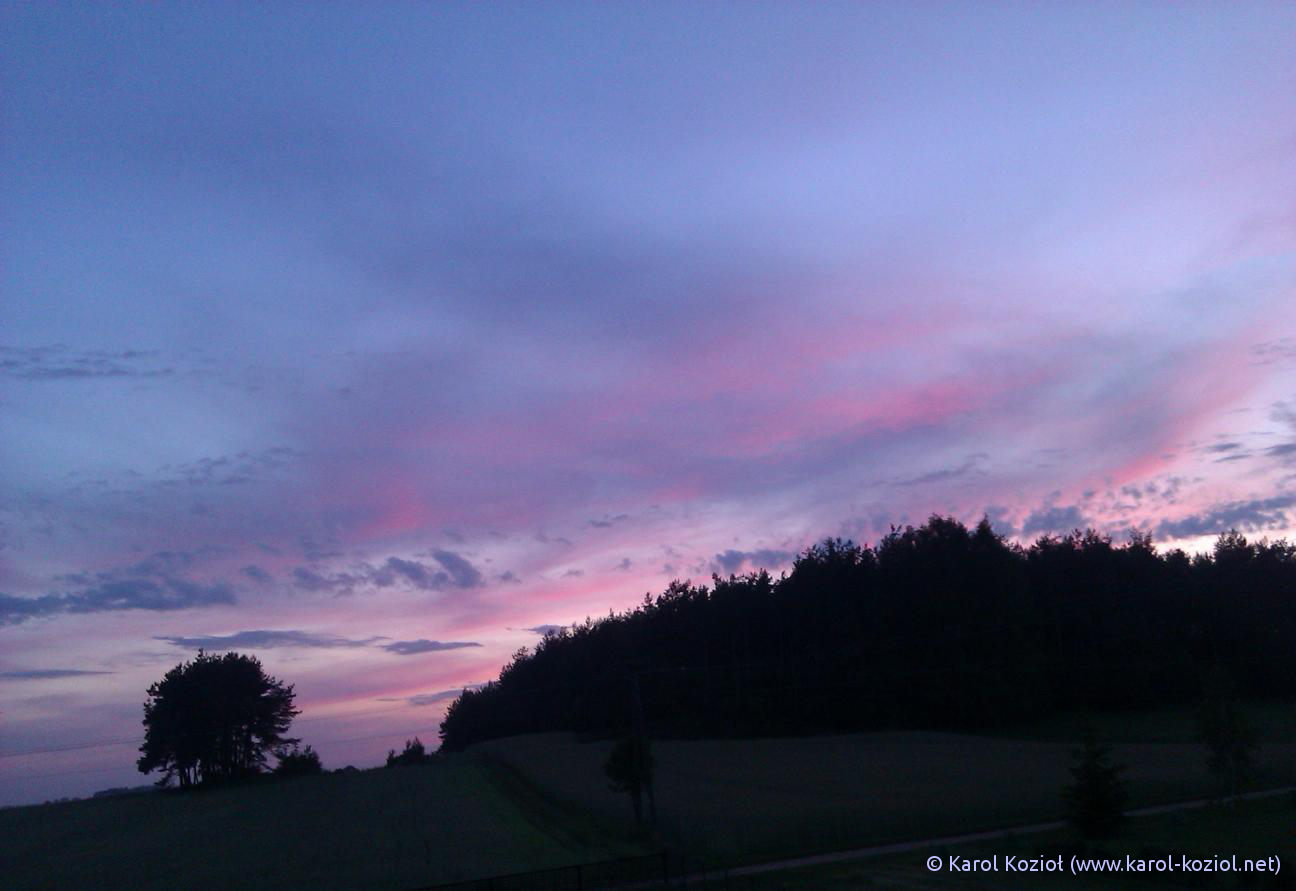
\includegraphics[width=0.68\textwidth]{sky.jpg}
\caption{sky}
\end{figure}


\lipsum[1]

\begin{description}
  \item[\ding{55}] asdfgh
  \item[\ding{55}] dsgfhf
  \item[\ding{55}] adgsfdhh
  \item[\ding{55}] sdgfhdgjfh
  \item[\ding{55}] asdf
\end{description}

\lipsum[1]
\lipsum[1]

\subsubsection{CCW}

\lipsum[1]

\subsubsection{\LaTeX}

本课程的期末报告我主要通过\LaTeX\ 完成。虽然此前我也用过\LaTeX\ 完成数学建模论文的书写,并获得了国家一等奖,但毫不夸张地说,本次经历让我对它的理解与掌握有了一个巨大的飞跃。

众所周知,常用\LaTeX\ 的同学很难习惯$Word$的过度灵活,而在没有模板的情况下使用它写论文又需要自行设计,耗时耗力。而此前,我在网上从未见过南开大学的\LaTeX\ 论文模板,于是我打算以此为契机,自己设计一个专属于南开大学的模板,并将之开源。虽然我可能没有什么机会再使用了,但相信这可以帮助到一些学弟学妹。

历时十多天,在不断的摸索与尝试中,我学会了如何设计版面、如何调整字体字号,如何修改各种主题色,如何高亮代码,如何调整标题和目录样式……

这些功能在本篇报告中只体现出了一部分,完整的模板我已经上传到了\href{https://github.com/brebalance/NKU-LaTeX-template.git}{\textit{我的$github$库}}中,并且后续还打算继续改进,在此欢迎老师给出批评与建议!

\subsection{学习方法收获}

\lipsum[1]

\section{感想与认识}

\lipsum[1]
\lipsum[1]
\lipsum[1]

\section{课程建议}

\lipsum[1]

\subsection{课堂讲授方面}

\lipsum[1]
\lipsum[1]

\subsection{实验任务方面}

\lipsum[1]
\lipsum[1]


\clearpage	
\section{参考文献}

\begin{flushleft}

[1]王华忠.工业控制系统及应用——$PLC$与人机界面.机械工业出版社,2019.

[2]王华忠.工业控制系统及应用——$PLC$与组态软件.机械工业出版社,2019.

[3]王欣.电气控制及$PLC$技术——$PLC$与组态软件.机械工业出版社,2019.

[4]课程中用到的$PPT$和实验指导书

\end{flushleft}









\end{document}          



